\documentclass{ctexart}

\title{LSM Tree实验报告}
\author{陈天予 519021910045}
\date{\today}
\usepackage{natbib}
\usepackage{graphicx}
\usepackage{enumitem}
\usepackage{subfigure}

\begin{document}

\maketitle

\section{背景介绍}
LSM Tree(Log-structure Merge Tree)数据结构,于1996年在Patrick O’Neil 等人的一篇论文提出。其通过SS-Table的多层储存结构,利用磁盘顺序读写的高效性,实现了性能极高的写操作。LSM Tree被广泛地在各种NoSQL中使用,比如HBase,LevelDB等。

\section{挑战}
\begin{enumerate}
  \item 持久化:之前写过的程序,数据结构都在内存中,很少涉及到文件的读写。LSM Tree通过客制化结构的SSTable实现持久化,需要通过二进制的方式来读写sst文件,因不熟悉c++相关的库函数而导致的bug就不少。
  \item sst文件的debug:由于sst文件在硬盘中,debug的过程中无法实时看到其中的数据,造成许多麻烦和障碍。最终写了一个peekSSTable的小程序扫描sst文件并输出debug信息,解决了debug时的困难。
  \item 一个难以复现的bug:在调试过程中,有一次发现一个难以复现的bug,复盘半天发现一个现象,如果两次debug时间间隔较长,这个bug就不会出现,反之就有很高机率出现。最终发现竟然是一个函数中忘记关闭文件,使得打开了过多的文件,在操作系统还未回收完这些fd前运行程序就有可能出现这个bug。
\end{enumerate}

\section{测试}

\subsection{测试环境}
AMD R7 3700x with SSD in Ubuntu 20.04 LTS

\subsection{性能测试}

\subsubsection{测试方法}
插入1000个随机大小在1 Byte到近2 MB的字符串(总数据量大约再1G左右),随后打乱所有keys,执行GET操作,再打乱所有keys,执行DELETE操作。重复上述方法连续测试三次,测试各方法的平均延时和吞吐。
\subsubsection{预期结果}
\begin{enumerate}
  \item 对每次测试:测试结果应该相近。
  \item 对PUT操作:随着插入数据量的增大,触发compaction的机率也越大,吞吐也越低。
  \item 对PUT操作:随着GET数据量的增大,吞吐也会越低。
  \item 对DELETE操作:由于DELETE操作相当于插入一个小字符串,所以对于不同大小的数据吞吐应该相同。但由于在del需要先判断key是否在数据库中,所以总体来说,其吞吐量趋势应与PUT类似,并稍低一些,因为其有可能触发compaction操作。
\end{enumerate}

\subsubsection{实际结果}
测试的结果如下:
\begin{verbatim}
    >>>>> Put Test <<<<<
    0...100...200...300...400...500...600...700...800...900...
    Average Delay For Different Size Data:
    0 ~ 0.25MB     : 3.94ms throughput: 254.00/s
    0.25MB ~ 0.5MB : 8.80ms throughput: 113.58/s
    0.5MB ~ 1MB    : 21.98ms throughput: 45.49/s
    1MB ~ 1.5MB    : 42.43ms throughput: 23.57/s
    1.5MB ~ 2MB    : 44.75ms throughput: 22.35/s
    
    Average Delay: 28.00ms, Average Throughput: 35.72/s
    Total Size Insert: 961MB
    
    >>>>> Get Test <<<<<
    Average Delay And Throughput For Different Size Data:
    0 ~ 0.25MB     : 98.67ms throughput: 10134.66/s
    0.25MB ~ 0.5MB : 137.13ms throughput: 7292.47/s
    0.5MB ~ 1MB    : 180.61ms throughput: 5536.77/s
    1MB ~ 1.5MB    : 238.53ms throughput: 4192.35/s
    1.5MB ~ 2MB    : 292.84ms throughput: 3414.80/s
    
    Average Delay: 203.35µs, Average Throughput: 4917.65/s
    
    >>>>> Delete Test <<<<<
    Average Delay And Throughput For Different Size Data:
    0 ~ 0.25MB     : 100.34ms throughput: 9965.85/s
    0.25MB ~ 0.5MB : 142.98ms throughput: 6993.74/s
    0.5MB ~ 1MB    : 192.80ms throughput: 5186.74/s
    1MB ~ 1.5MB    : 262.21ms throughput: 3813.78/s
    1.5MB ~ 2MB    : 327.54ms throughput: 3053.05/s
    
    Average Delay: 221.23µs, Average Throughput: 4520.18/s
    
    >>>>> Summary <<<<<
    It takes 28s to complete the test.
\end{verbatim}

\subsubsection{结果分析}
测试结果与预期相符。不足之处在于PUT操作的测试颗粒度不够,对于小数据量的测试不够完全。
\begin{figure}
  \centering
  \subfigure[GET]
  {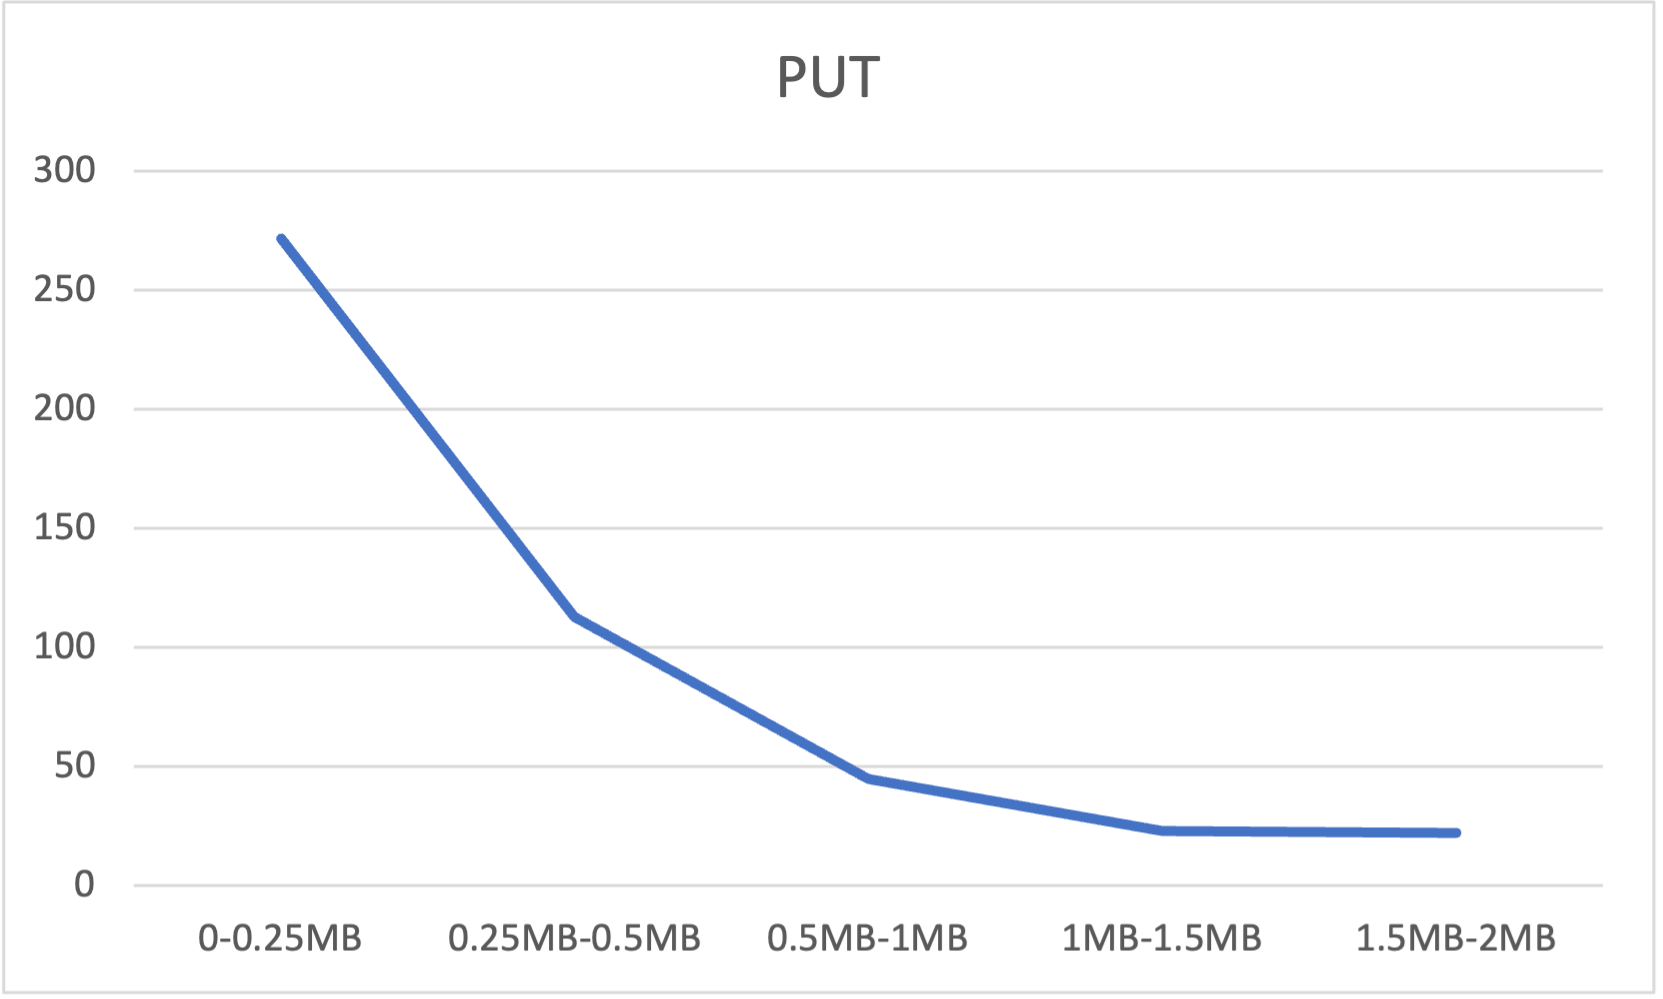
\includegraphics[width=4cm]{GET.png}}
  \subfigure[PUT \& DELETE]
  {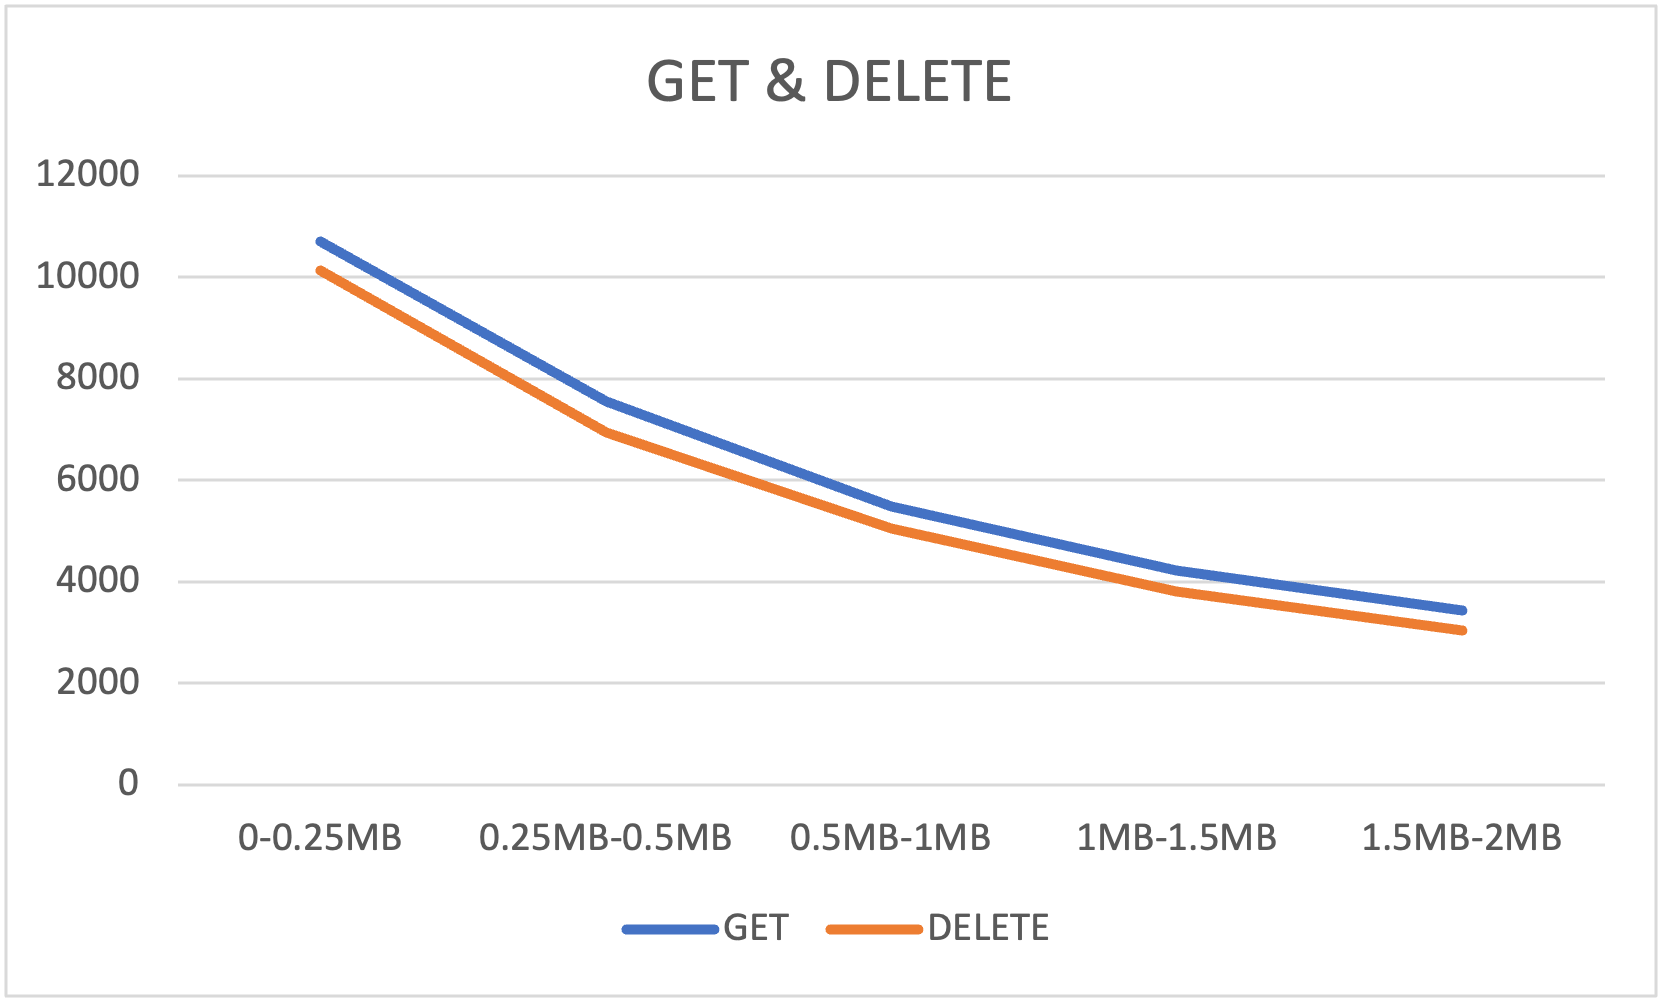
\includegraphics[width=4cm]{PUT-DELETE.png}}
  \caption{各操作对不同数据量的吞吐}
\end{figure}


\subsection{索引缓存与Bloom Filter的效果测试}

\subsubsection{测试方法}
测试脚本与性能测试相同,不同版本的代码存放在不同的git分支中,其中无缓存版本对应着naive分支,缓存索引信息的版本对应着index\_cached分支,完全版本在master中。

\subsubsection{预期结果}
三种测试中GET操作的平均时延应有显著差距,但同种测试之间对不同数据大小的时延变化趋势应与性能测试中的相同。

\subsubsection{实际结果}
因篇幅限制,实际输出放在了cache\_test.md中,这里只放图表。


\end{document}